%\documentclass[tikz,border=5pt]{standalone}
\begin{document}
	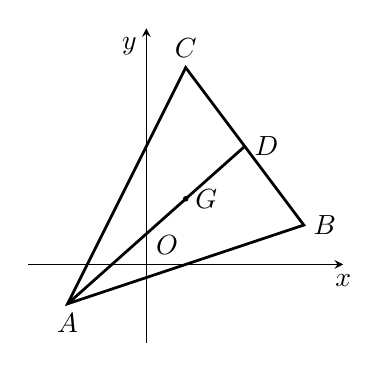
\begin{tikzpicture}[>=stealth, scale=0.5]
		% 绘制坐标轴
\draw[->] (-3,0) -- (5,0) node[below] {$x$}; % x 轴(带箭头与标签)
\draw[->] (0,-2) -- (0,6) node[below left] {$y$}; % y 轴(带箭头与标签)
\node at (0,0) [above right] {$O$}; % 原点 $O$ 的标签

% 定义各关键点坐标(可根据图形比例调整)
\coordinate (A) at (-2,-1);   % 点 $A$
\coordinate (B)  at (4,1);    % 点 $B$
\coordinate (C) at (1,5);    % 点 $C$
\coordinate (G) at (1,5/3);    % 点 $G$ 计算重心G的坐标 (重心坐标 = 三个顶点坐标的平均值)
\coordinate (D) at (2.5,3);    % 点 $D$

% 绘制连线
\draw [line width=1pt] (A) -- (B) -- (C) -- cycle; % 绘制三角形
\draw [line width=1pt] (A) -- (D);  % 绘制三条中线(从顶点到对边中点)

% 标记各点的标签 实心圆点
\fill (G) circle (2pt) node [right] {$G$};  % 带标签的实心点
\node at (A) [below] {$A$}; 
\node at (B) [right] {$B$}; 
\node at (C) [above] {$C$}; 
\node at (D) [right] {$D$}; 

	\end{tikzpicture}
\end{document}
